
\chapter{Introduction}
\label{sec:org76eb342}
\section{Motivation}
\label{sec:org37e5d53}
The discoveries in quantum physics during the last century opened multiple questions due to the observation of extraordinary behaviours that are far from the classical physics we are used to.
The answers of these questions as well as another field's investigations rely on the simulation of Nature.
In order to understand our world we need to simulate instances of it, but the simulation of Nature itself requires a huge computational power that is intractable for classical computers.
At the same time, we are witnesses of the Moore's law halt; we are reaching the limit in transistor sizes.
While trying to make them smaller, quantum phenomena appear making impossible a transistor behaviour.
During the last century Feynman had the idea of getting advantage of the unexplained but controllable quantum phenomena.
He noticed that this quantum phenomena that would stop the development of smaller transistors and, therefore, powerful chips, actually could be used to get much more computational power. He was the first to introduce the idea of building a quantum computer to simulate quantum mechanics in 1982.


Since then, research on quantum computing has been mostly focusing on the development of quantum technologies and quantum algorithms. In order to bridge the gap between them, the Quantum Computer Architecture Lab at Delft University of Technology proposed a full-system stack, an architecture for a quantum computer \cite{Fu_2016}. As shown in Figure  \ref{fig:system_stack} it consists of quantum algorithms that can be expressed expressed by a high-level programming language and then compiled to a series of instructions. In the microarchitecture, those instructions are translated into signals that are sent to operate on the qubits.  



As a part of this full-system stack, and when targeting a real quantum processor,  quantum algorithms need to be adapted to the constraints  of the quantum chip; they need to be mapped.
%Our QCA lab at TU Delft University of Technology develop a general architecture for quantum computers \cite{Fu_2016} that follow a process which steps can be see in Fig. \ref{fig:system_stack}.
%This process goes from the algorithms description -- upper layer in the figure -- to the set of instructions that are sent as hardware dependent signals  -- lower layer -- to the hardware interface that controls the quantum chip.


\begin{figure}[htbp]
\centering
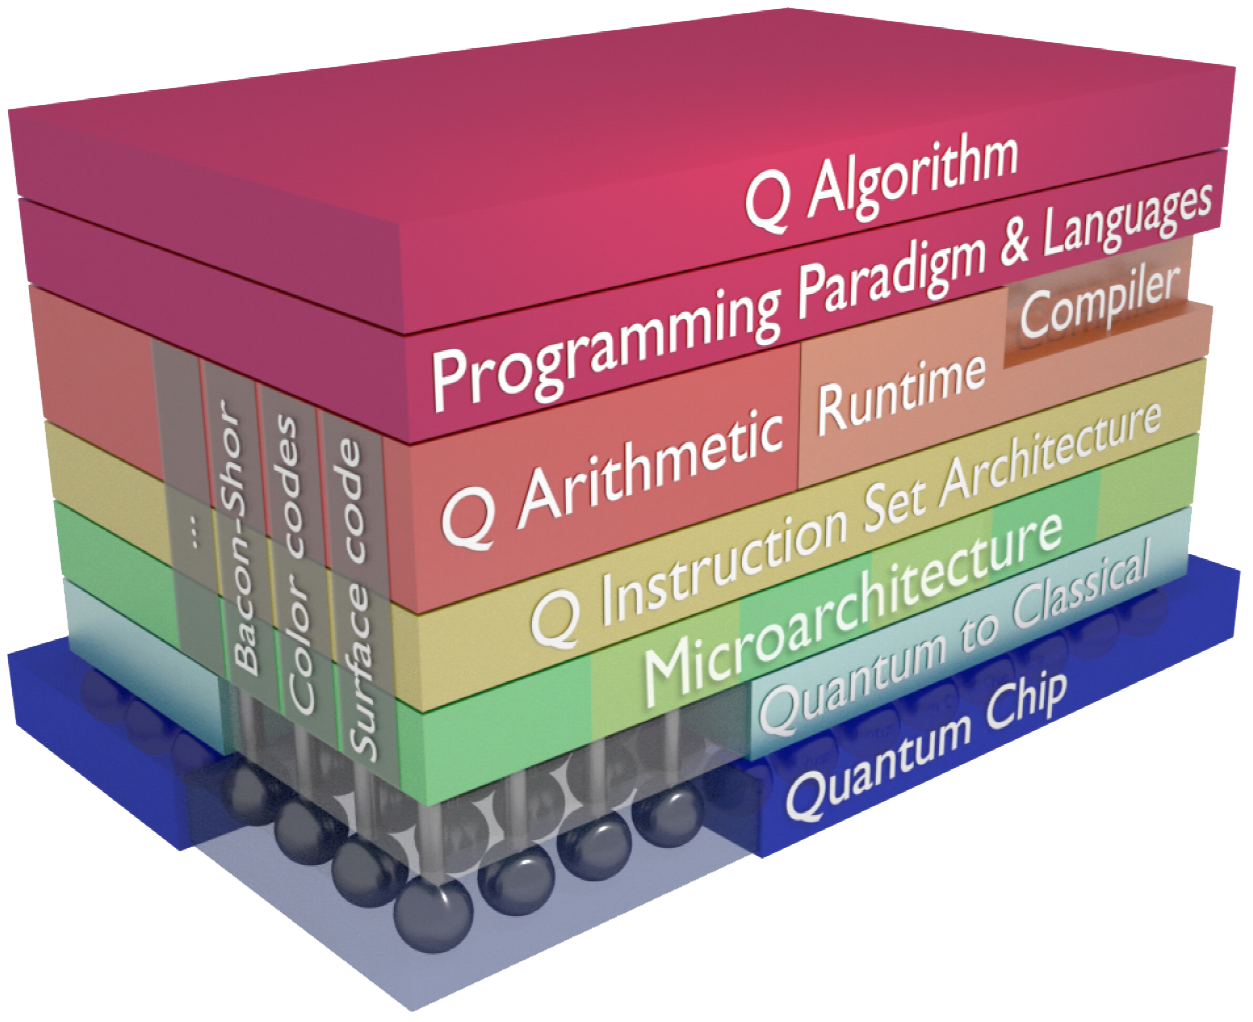
\includegraphics[width=0.5\textwidth]{figures/system_stack.png}
\caption{\label{fig:system_stack}
Full stack implementation \cite{Fu:2017:EMS:3123939.3123952}}
\end{figure}

\section{Problem Statement}
\label{sec:org81811d9}
Quantum algorithms are represented as quantum circuits when the circuit model of computation is adopted. Quantum circuits consist of quantum bits and gates operating on them.
This representation (at high-levels of the system stack) is hardware agnostic; that is, it does not take into account the possible constraints of the quantum chip. Therefore, mapping models are required to have a version of the quantum algorithm adapted to the quantum device and that can be executed on it. Note that, one of main constraint in current quantum chips is the reduced connectivity between the qubits that limits their interaction to only nearest- neighbours.


The mapping process results in an increase of the number of gates of the circuit and/or the circuit depth (or circuit latency), affecting the reliability of the algorithm. As qubits decohere and gates are error prone, the higher the number of operations or the higher the circuit depth, the higher the probability of having an error during computation.  Therefore, mapping models require an optimization process in search of the best circuit version that is executable on a given device and still produces `good' results.

Most of the works done about the mapping task optimize in terms of two parameters, either the number of added operations in the adapted version of the circuit or the latency added to the circuit. Moreover, these works asses the quality of their mapping algorithms based on one of those two metrics. It is clear that both parameters should be as small as possible. However, these metrics are not complete and do not give nay information on how the mapping affects the algorithm's reliability.

Given this scenario, the aim of this thesis is to propose different metrics that show how the algorithm's reliability is affected by the mapping process.  To this purpose, we will focus on the fidelity  and the probability of success and how they relate with the quantum volume and other metrics such are number of gates, number of two-qubit gates and circuit depth.

\section{Structure of the thesis}
\label{sec:orgdf4cd06}
This thesis follows the structure described below:

In \hyperref[sec:org9b8733c]{chapter 2}, a background on the quantum computing field is given. 
We also explain the insights of the mapping task, as well as current state-of-the-art in this field.
Finally, a description of the most used mapping metrics is described.

In \hyperref[sec:org0c87802]{chapter 3}, we describe the constrains of the quantum chip that we target to map quantum algorithms on.
Constrains that we need to take into account in our mapping model, which we describe afterwards.
This chapter concludes with an explanation of the new mapping metrics we will investigate.

In \hyperref[sec:org17c0cef]{chapter 4}, we explain the process we followed to evaluate the mapping metrics. 
First, we select a set of quantum algorithms as benchmarks.
This benchmarks will be mapped following the constrains of the quantum chip and then simulated.
This process will be led by the analysis framework we developed and that we describe in detail in this chapter.

In \hyperref[sec:orgaed8c93]{chapter 5}, the results are presented and, finally, in \hyperref[sec:org7d44186]{chapter 6}, we conclude the thesis and we set the future work for this topic.